\documentclass{elsarticle}

%%%%%%%%%%%%%%%%%%%%%%%%%%%%%% User specified LaTeX commands.
%\usepackage[utf8]{inputenc}
\usepackage{amssymb}
%%%%%%%%%%%%%%%%%%%%%%%%%%%%%% User specified LaTeX commands.
\newcommand{\ie}{\textit{i.~e.} }
\newcommand{\cref}{c^{\ominus}}
%\newcommand{\cs}{c_{s}}
\newcommand{\kT}{k_\mathrm{B}T}
\newcommand{\kB}{k_\mathrm{B}}
\newcommand{\lb}{l_\mathrm{B}}
\newcommand{\NA}{N_{\mathrm{A^-}}}
\newcommand{\muna}{\mu_\mathrm{Na^+}}

\newcommand{\mucl}{\mu_\mathrm{Cl^-}}
\newcommand{\muca}{\mu_\mathrm{Ca^{2+}}}
\newcommand{\muh}{\mu_\mathrm{H^+}}
\newcommand{\mua}{\mu_\mathrm{A^-}}
\newcommand{\muha}{\mu_\mathrm{HA}}
\newcommand{\muoh}{\mu_\mathrm{OH}}

\newcommand{\cna}{c_\mathrm{Na^+}}
\newcommand{\ccl}{c_\mathrm{Cl^-}}
\newcommand{\cca}{c_\mathrm{Ca^{2+}}}
\newcommand{\ch}{c_\mathrm{H^+}}
\newcommand{\cp}{c_\mathrm{p}}
\newcommand{\nna}{n_\mathrm{Na^+}}
\newcommand{\ncl}{n_\mathrm{Cl^-}}
\newcommand{\Nna}{N_\mathrm{Na^+}}
\newcommand{\Ncl}{N_\mathrm{Cl^-}}

\newcommand{\ncleq}{\widetilde{N}_\mathrm{Cl^-}}
\newcommand{\nca}{N_\mathrm{Ca^{2+}}}

\newcommand{\superin}{^\mathrm{in}}
\newcommand{\subin}{_\mathrm{in}}
\newcommand{\subi}{_\mathrm{i}}

\newcommand{\gel}{^\mathrm{gel}}
\newcommand{\tot}{^\mathrm{tot}}
\newcommand{\out}{^{\mathrm{out}}}
\newcommand{\coh}{c_\mathrm{OH}}
\newcommand{\bulk}{^{\mathrm{b}}}
\renewcommand{\H}{\mathrm{H^+}}
\newcommand{\A}{\mathrm{A^-}}
\newcommand{\AH}{\mathrm{AH}}
%%%%%%%%%%%%%%%%%%%%%%%%%%%%%% LyX specific LaTeX commands.
%% A simple dot to overcome graphicx limitations
\newcommand{\lyxdot}{.}
\newcommand{\todoi}[1]{\todo[inline]{#1}}
\setuptodonotes{fancyline, color=blue!30, size=\tiny}

\newcommand{\cl}{\mathrm{Cl^-}}
\newcommand{\br}{\mathrm{Br^-}}
\newcommand{\na}{\mathrm{Na^+}}
\newcommand{\h}{\mathrm{H^+}}
\newcommand{\ka}{\mathrm{K^+}}
\newcommand{\oh}{\mathrm{OH^-}}
\newcommand{\ca}{\mathrm{Ca^{2+}}}
\newcommand{\mg}{\mathrm{Mg^{2+}}}
\newcommand{\so}{\mathrm{SO_4^{2-}}}

\newcommand{\EI}{E_{\mathrm{I}}}
\newcommand{\EII}{E_{\mathrm{II}}}
\newcommand{\SI}{S_{\mathrm{I}}}
\newcommand{\SII}{S_{\mathrm{II}}}
\newcommand{\NI}{N_{\mathrm{I}}}
\newcommand{\NII}{N_{\mathrm{II}}}
\newcommand{\VI}{V_{\mathrm{I}}}
\newcommand{\VII}{V_{\mathrm{II}}}
\newcommand{\FI}{F_{\mathrm{I}}}
\newcommand{\FII}{F_{\mathrm{II}}}
\newcommand{\nnaI}{N^{\na}_{\mathrm{I}}}
\newcommand{\nclI}{N^{\cl}_{\mathrm{I}}}
\newcommand{\nnaII}{N^{\na}_{\mathrm{II}}}
\newcommand{\nclII}{N^{\cl}_{\mathrm{II}}}




\newcommand{\Ka}{K_{\mathrm{A}}}
\newcommand{\pKa}{\mathrm{p}\Ka}
\newcommand{\pK}{\mathrm{p}K}
\newcommand{\pH}{\mathrm{pH}}
\newcommand{\mol}{\mathrm{mol}}
\newcommand{\molperl}{\mathrm{mol/l}}
\newcommand{\kg}{\mathrm{kg}}
\newcommand{\res}{^{\mathrm{res}}}
\newcommand{\pHres}{\pH\res}
\newcommand{\pHgel}{\pH\gel}
\newcommand{\cs}{c_{\mathrm{s}}}
%\newcommand{\cs}{c_{\mathrm{salt}}}
\newcommand{\csres}{\cs\res}
%\newcommand{\Vgel}{V\gel}
%\newcommand{\Vgel}{V_\mathrm{gel}}
\newcommand{\Vgel}{V}
\newcommand{\Ngel}{N_\mathrm{gel}}
%\newcommand{\Vgeleq}{\widetilde{V}_\mathrm{gel}}}
\newcommand{\Pgel}{P_\mathrm{gel}}
\newcommand{\Pres}{P_\mathrm{res}}
\newcommand{\Pout}{P_\mathrm{out}}
\newcommand{\Vout}{V_\mathrm{out}}
%\newcommand{\Vbox}{V_\mathrm{box}}
\newcommand{\Vbox}{V_0}
\newcommand{\PE}{polyelectrolyte{}}

\newcommand{\reffig}[1]{Figure~\ref{#1}}
\newcommand{\refeq}[1]{Equation~\ref{#1}{}}
\usepackage{afterpage}
\newcommand\blankpage{%
    \null
    \thispagestyle{empty}%
    \addtocounter{page}{-1}%
    \newpage}


\newcommand{\mytitle}{Gibbs ensemble for \PE{} hydrogel}
\newcommand{\etal}{\textit{et al.}{}}

\@ifundefined{showcaptionsetup}{}{%
 \PassOptionsToPackage{caption=false}{subfig}}
\usepackage{subfig}

\usepackage[margin=2.5cm]{geometry}% by courtesy of Mico
\begin{document}
\begin{frontmatter}{}


\title{\mytitle}

%\title{The \PE{} hydrogels as draw agents for desalination of solutions with multivalent ions}

%\tnotetext[t1]{This document is a collaborative effort.}
%\tnotetext[t2]{The second title footnote which is a longer longer than the first one and with an intention to fill in up more than one line while formatting.}

    \author[cuni,imc]{Michail Laktionov}
    \ead{michail.laktionov@natur.cuni.cz}
    \ead[url]{http://www.physchem.cz/}
    \author[cuni]{Oleg V. Rud}
    \author[cuni]{Lucie~Nova}
    %\author[cuni]{Peter~Kosovan}
    \author[cuni]{Filip~Uhlik}


    \address[cuni]{Department of Physical and Macromolecular Chemistry, Faculty of Science, Charles University in Prague, Hlavova 8, Praha 2 128 00, Czech Republic}
    \address[imc]{Institute of Macromolecular Compounds of Russian Academy of Sciences, 199004, Bolshoy pr. 31, Saint-Petersburg, Russia}




\begin{abstract}
By this article we model compression of \PE{} hydrogel in equilibrium with small volume of salty aqueous solution.
We show that the the change of the hydrogel volume affects the salinity of the solution. The decrease of the gel volume decreases the solution and vice versa the swelling of the gel increases the surrounding solution. 
This effect can be employed for water desalination ...
\end{abstract}

\end{frontmatter}{}

\section{Theory behind the simulation\label{sec: theory}}

\reffig{fig:diamond} presents a diamond-like polymer network inserted in a simple cubic simulation box of volume $V_{\mathrm{box}}$ with periodic boundaries.
The network consists of $16$ linear \PE{} chains, each chain comprising $30$ monomer units.
Each unit is able to change its ionization state from charged to neutral and vice versa according to the ionization equilibrium.
The mobile ions ($\na$, $\cl$ and $\ca$) are present in certain amount such that they fulfill the electroneutrality condition.

We model the network in equilibrium with the bulk of aqueous solution.
In order to keep the equilibrium conditions we consider three processes to occur:

\begin{enumerate}
	\item the thermal movement of all segments in simulation box (Langevin dynamics);
	\item the transfer of ions between two vessels:
        \item the change of ratio between volumes of the two vessels emulationg the piston applying certain pressure to one of the vessels:
%\todoi{We shall get rid of $\so$ ions and mention it in the inroduction. The reason is that their concentration is small, and they do not enter the hydrogel }
\end{enumerate}

All three processes occur simultaneously in real systems, however, we simulate them alternating each other in stop-run mode in a random order.
\begin{figure}[h]
    \centering
    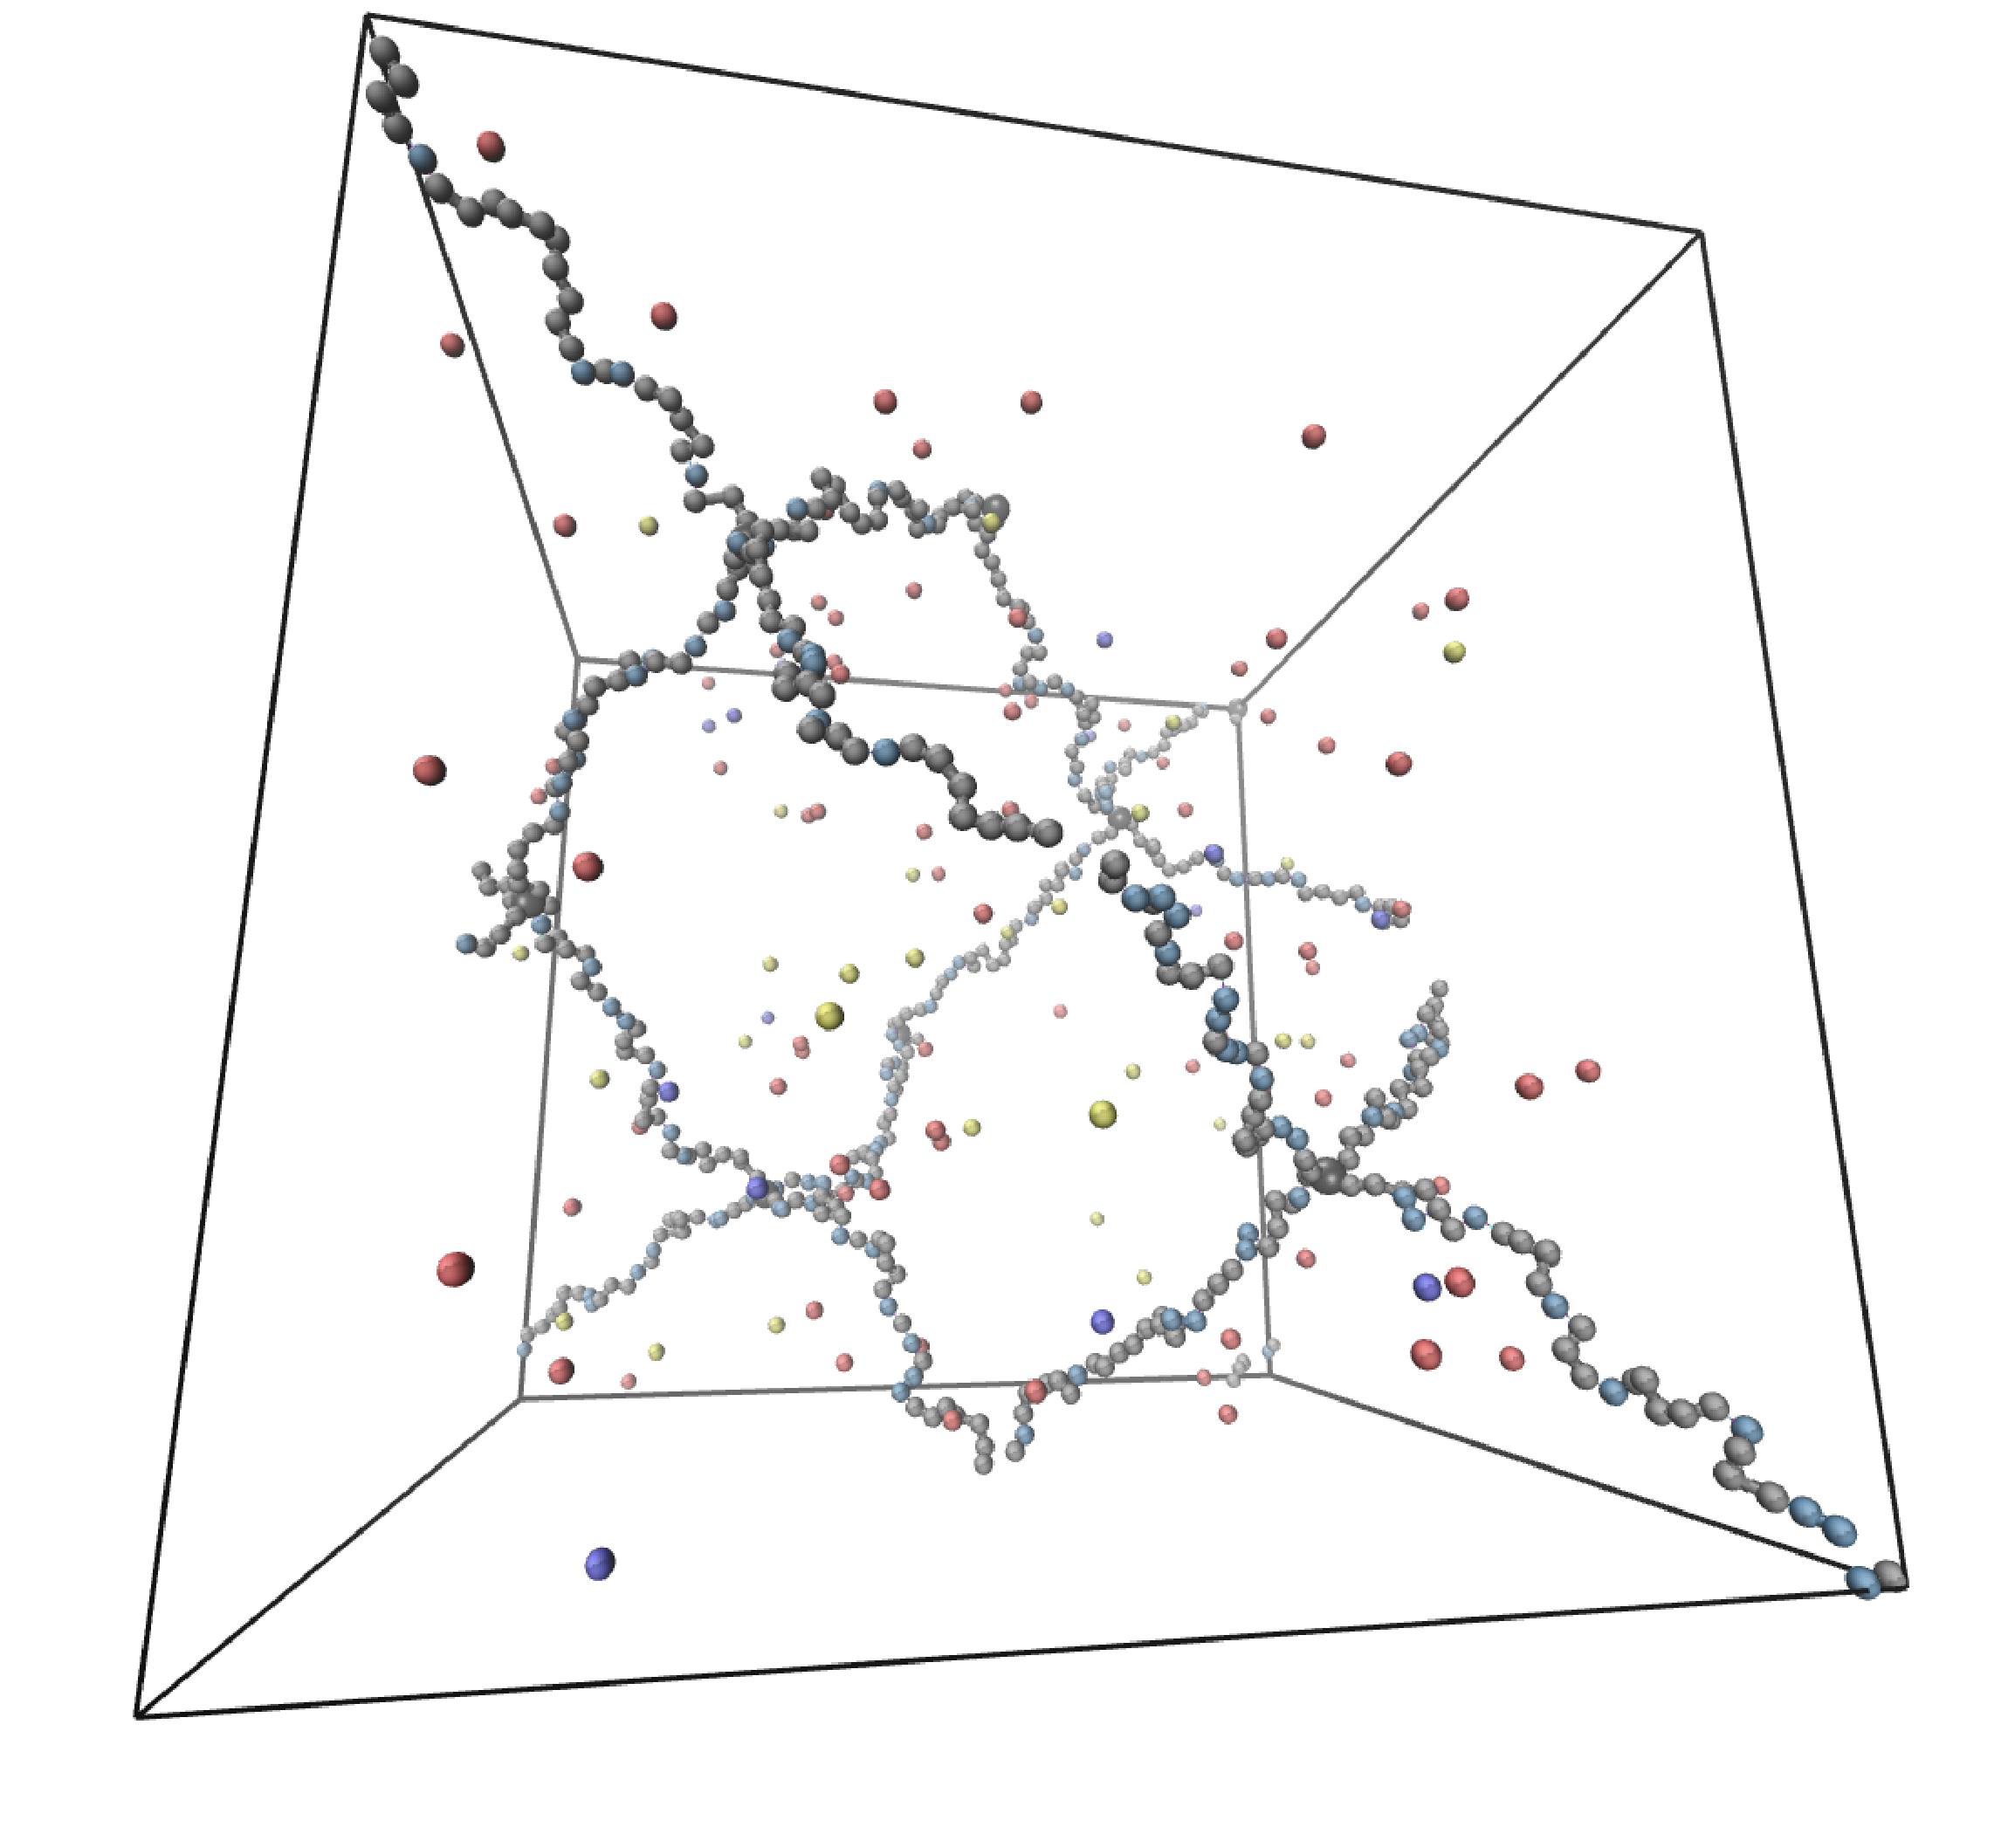
\includegraphics[width=0.5\columnwidth]{{figures/vmdscene}.pdf}
    \caption{
       	Diamond-like network in the simulation box. 
	Color code represents the individual ion types
	(red: $\na$, blue: $\cl$, yellow: $\ca$) and
        the hydrogel (gray: neutral segment ($\AH$), cyan: charged segment ($\A$)).
    }
    \label{fig:diamond}
    %in order to make snapshot use file snapshot.py
    % in order to edit the existing snapshot use file data/gel_MPC30_box_l53.0_pK7.00_pH7.00_pCl2.00_pCa2.94_lB0.0.vmd
\end{figure}
\todo{remove $\ca$ ions from snapshot}
\subsection{Langevin dynamics\label{MD}}

We use three types of interactions, \ie bonded interactions, short-range non-bonded interactions and electrostatic interactions.

We use Finite extension nonlinear elastic (FENE) potential~\refeq{eq:fene} to account for the bonding interactions.
%The potential accounts for nonlinear elastic extensions and as a consequence, the simulation is not constrained too much.
\begin{equation}\label{eq:fene}
    V_\mathrm{FENE}(r) = -\frac{1}{2} K \Delta r_\mathrm{max}^2\ln \left[ 1 - \left(\frac{r-r_0}{\Delta r_\mathrm{max}} \right)^2 \right ],
\end{equation}
where $K$ is the magnitude of symmetric interaction between two segments,
$\Delta r_{\mathrm{max}}$ is the maximal stretching length of the bond and $r_0$ is the equilibrium bond length.
In our simulations we set $K = 10 \kT/\sigma^{2}$, $\Delta r_{\mathrm{max}} = 2 \sigma$ and $r_0 = 1.0\sigma$~\cite{Jin2007}.

We model the non-bonded interactions using truncated Lennard-Jones interaction potential.
This potential imposes strong repulsion between all particles at short distances:
\begin{equation}
    \begin{split}\label{eq:LJ}
        V_\mathrm{LJ}(r) =
        \begin{cases}
            4 \varepsilon \left( \left(\cfrac{\sigma}{r}\right)^{12}
            - \left(\cfrac{\sigma}{r}\right)^6\right)
            & \mathrm{if~} r < r_\mathrm{cut}\\
            0
            & \mathrm{elsewhere}
        \end{cases},
    \end{split}
\end{equation}
where $r$ is the interparticle distance,
$\sigma = 0.35 \mathrm{nm}$ is the characteristic size of the particles,
$\varepsilon$ is the depth of the potential well in $\kT$ units and $r_\mathrm{cut}$ is the cut-off distance beyond which the potential is set zero.

We model the long range electrostatic interactions by the Coulomb potential:
\begin{equation}
    V_{\mathrm{EL}}=\lb\kT \cfrac{q_{1}q_{2}}{r},
\end{equation}
where $\lb$ is Bjerrum length. We set $\lb = 2\sigma = 0.7 \mathrm{nm}$ which corresponds to water at $T=300 \mathrm{K}$.


We use Langevin thermostat, \ie
we add two additional terms to force in equation of motion
\begin{equation}
f_i =  -\gamma v_i(t)+\sqrt{2\gamma \kT }\eta_i(t),
\end{equation}
where the first term correspond to constant friction with $\gamma$ being a friction coefficient, and the second one corresponds to random thermal force with $\eta_i$ being a normally distributed random number (see for details \cite{Grest1986}).

%where $\gamma$ is the friction coefficient and .
%\todo{there is friction and there is random force ballanced by fluctiation dissipation theorem so that it is stationary}
%which causes the decrease of the particles' velocities.
%This is implemented by addition of two corresponding terms to the particles' equations of motion, namely
%\todo{usually -gamma v to keep gamma>0}
%where the first term correspond to 



%\paragraph{Units} % apart from cref reference all references are in the text. Do we need cref?
%By setting up the interaction potentials we defined the system of units.
%We have chosen the unit of length being based on the Bjerrum length in water at room temperature, $l_B \simeq 7$nm, and $\sigma=0.5l_B = 0.35$.
% % %Then the unit of concentration is $\cref=(\sigma^{3}\NA1000)^{-1}$mol/l. % % % do we need to say that?
%We set the energy unit to be $\varepsilon = \kT$.


\section{Sampling in the Gibbs ensemble\label{sec: sampling the gibbs ensemble}}
All thermal moves are frozen during the sampling of the ion pairs exchange.
The system represents the ensemble with constant number of particles distributed between two vessels (I) and (II).

In the following paragraph we derive the criteria for sampling of the ion exchange equilibrium.
\paragraph{Gibbs canonical ensemble}
Let us first consider the total free energy of both vesselsassuming that we have only particles of a single type:
\begin{equation}
    F=\left(E_{I}-TS_{I}\right) + \left(E_{II}-TS_{II}\right) \label{eq:F-gibbs}
\end{equation}
where $E$ is internal energy, $T$~--- temperature, $S$~--- entropy.

%Our model system represents a finite volume $V$ which exchanges particles with the bath of infinite volume.
%The infinity of the volume means, that the particle exchange between the system and the bath does not influence on the chemical potentials in the bath.
%Such ensemble is called grand canonical ensemble; the free energy in this ensemble, the Landau potential, is
The entropy $S$ is given by the Boltzmann formula~\cite{Nagle2004}:
\begin{equation}
    S=\kB\ln\frac{V^{N}}{N!}\label{eq:entropy}
\end{equation}
%\todo{for partiles without interactions}
where $N$ is a number of particles in corresponding vessel.
This formula accounts for two contributions:
\begin{enumerate}
    \item the combinatorial entropy $S_{c}=-\kB\ln N!$ which reflects the freedom of choice among $N$ particles
    \item the mixing entropy $S_{m}=\kB N\ln V$ which reflects the freedom to place the chosen particle randomly within the simulation box. 
\end{enumerate}
$V$ is the unitless volume, \ie the volume measured in units of $\sigma^3$. 
Thus \refeq{eq:F-gibbs} turns to 
%\todo{this is not reason, moreover A.10 is already wrong as for units}
\begin{equation}
    F=\EI-\kT\ln\frac{\VI^{\NI}}{\NI!}\ + \ \EII-\kT\ln\frac{\VII ^{\NII}}{{\NII} !}
\label{eq: F_gibbs}
\end{equation}
When a single particle transferred from the vessel (I) to the  vessel (II) the free energy in vessel (I) changes 
\begin{equation}
\Delta \FI = \Delta \EI+\kT\ln\frac{\VI^{\NI}}{\NI !} - \kT\ln\frac{\VI^{\NI-1}}{(\NI-1)!}=\Delta \EI + \kT\ln\frac{\VI}{\NI}
\end{equation}
whwereas the free energy change in (II) vessel is
\begin{equation}
\Delta \FII = \Delta \EII+\kT\ln\frac{\VII^{\NII}}{\NII !} - \kT\ln\frac{\VII^{\NII+1}}{(\NII+1)!}=\Delta \EII + \kT\ln\frac{\NII+1}{\VII}
\end{equation}
Thus the total change of free energy will be 
\begin{equation}
\Delta F = \Delta \EI+\Delta \EII+\kT\ln\frac{\VI}{\VII}\frac{\NII+1}{\NI}
\end{equation}
Introducing $\xi=\pm 1$, which reflects the direction of movement of particle, $\xi$= +1 if the particles moves from vessel (I) to vessel (II), and $\xi=-1$ if the particles moves backwards, then the previous formula transfers to 

\begin{equation}
\Delta F = \Delta E_{tot}+\kT\xi\ln\frac{\VI}{\VII}\frac{\NII+\theta(\xi)}{\NI+\theta(-\xi)}
\end{equation}
where $\theta(x)$ is the Heaviside function.

In order to keep electroneutrality of the system we transfer particles by elctroneutral pairs. 
Accounting for two types of particles which are moved all the time together the previous formula translates to the following
\begin{equation}
\Delta F = \Delta E_{tot}+\kT\xi\left(\ln\frac{\VI}{\VII}\frac{\nnaII+\theta(\xi)}{\nnaI+\theta(-\xi)}    + 
							    \ln\frac{\VI}{\VII}\frac{\nclII+\theta(\xi)}{\nclI+\theta(-\xi)}             \right)
\end{equation}
or
\begin{equation}
\Delta F = \Delta E_{tot}+\kT\xi\ln\left(\left(\frac{\VI}{\VII}\right)^2\prod_{i}\frac{\NII^i+\theta(\xi)}{\NI^i+\theta(-\xi)}\right) 
\end{equation}
where $i$ runs over the ion types $i\in\{\na,\ \cl\}$.

In order to simulate an ensemble composed of two vessels exchanging particles with each other we need to perform the following Monte Carlo procedure \cite{Frenlkel2002_book, SilvaFernandes2015a, Panagiotopoulos1988b}
\begin{enumerate}
	\item we propose the new configuration of the system by removing ion pair from one vessel and inserting it to another
	\item we accept the new configuration if
	\begin{equation}
        \mathcal{R}^{\xi}<e^{\Delta F/\kT}\label{eq: GC acceptance}
	\end{equation}
\end{enumerate}
where $\mathcal{R}$ is uniformly distributed random number in range between $0$ and $1$.


\section*{Acknowledgments}

This research was supported by the Czech Science Foundation (grant 19-17847Y) (OR, LN, AK),
Government of Russian Federation, grant number 14.W03.31.0022. % is it really necessary to add this aknowledgement? Who is paid from this project?
AK thanks the Grant Agency of Charles University for support (project 318120).
Computational resources were supplied by the project "e-Infrastruktura CZ" (e-INFRA LM2018140) provided within the program Projects of Large Research, Development and Innovations Infrastructures.

\bibliographystyle{plain}
\bibliography{gibbs}


\newpage
\pagebreak

\end{document}
